
%% ou-crc-phd-students-conf.tex
%% V2.0
%% 2015/05/20
%% by Andrea Franceschini and Theo Georgiou
%%
%% BASED ON
%%
%% bare-conf.tex
%% V1.3
%% 2007/01/11
%% by Michael Shell
%% See:
%% http://www.michaelshell.org/
%% for current contact information.
%%
%% This is a skeleton file demonstrating the use of IEEEtran.cls
%% (requires IEEEtran.cls version 1.7 or later) with an IEEE conference paper.
%%
%% Support sites:
%% http://www.michaelshell.org/tex/ieeetran/
%% http://www.ctan.org/tex-archive/macros/latex/contrib/IEEEtran/
%% and
%% http://www.ieee.org/

%%*************************************************************************
%% Legal Notice:
%% This code is offered as-is without any warranty either expressed or
%% implied; without even the implied warranty of MERCHANTABILITY or
%% FITNESS FOR A PARTICULAR PURPOSE! 
%% User assumes all risk.
%% In no event shall IEEE or any contributor to this code be liable for
%% any damages or losses, including, but not limited to, incidental,
%% consequential, or any other damages, resulting from the use or misuse
%% of any information contained here.
%%
%% All comments are the opinions of their respective authors and are not
%% necessarily endorsed by the IEEE.
%%
%% This work is distributed under the LaTeX Project Public License (LPPL)
%% ( http://www.latex-project.org/ ) version 1.3, and may be freely used,
%% distributed and modified. A copy of the LPPL, version 1.3, is included
%% in the base LaTeX documentation of all distributions of LaTeX released
%% 2003/12/01 or later.
%% Retain all contribution notices and credits.
%% ** Modified files should be clearly indicated as such, including  **
%% ** renaming them and changing author support contact information. **
%%
%% File list of work: IEEEtran.cls, IEEEtran_HOWTO.pdf, bare_adv.tex,
%%                    bare_conf.tex, bare_jrnl.tex, bare_jrnl_compsoc.tex
%%*************************************************************************

% *** Authors should verify (and, if needed, correct) their LaTeX system  ***
% *** with the testflow diagnostic prior to trusting their LaTeX platform ***
% *** with production work. IEEE's font choices can trigger bugs that do  ***
% *** not appear when using other class files.                            ***
% The testflow support page is at:
% http://www.michaelshell.org/tex/testflow/



% Note that the a4paper option is mainly intended so that authors in
% countries using A4 can easily print to A4 and see how their papers will
% look in print - the typesetting of the document will not typically be
% affected with changes in paper size (but the bottom and side margins will).
% Use the testflow package mentioned above to verify correct handling of
% both paper sizes by the user's LaTeX system.
%
% Also note that the "draftcls" or "draftclsnofoot", not "draft", option
% should be used if it is desired that the figures are to be displayed in
% draft mode.
%
\documentclass[conference,a4paper]{IEEEtran}
% If IEEEtran.cls has not been installed into the LaTeX system files,
% manually specify the path to it like:
% \documentclass[conference]{../sty/IEEEtran}

\usepackage{flushend}



% Some very useful LaTeX packages include:
% (uncomment the ones you want to load)


% *** MISC UTILITY PACKAGES ***
%
%\usepackage{ifpdf}
% Heiko Oberdiek's ifpdf.sty is very useful if you need conditional
% compilation based on whether the output is pdf or dvi.
% usage:
% \ifpdf
%   % pdf code
% \else
%   % dvi code
% \fi
% The latest version of ifpdf.sty can be obtained from:
% http://www.ctan.org/tex-archive/macros/latex/contrib/oberdiek/
% Also, note that IEEEtran.cls V1.7 and later provides a builtin
% \ifCLASSINFOpdf conditional that works the same way.
% When switching from latex to pdflatex and vice-versa, the compiler may
% have to be run twice to clear warning/error messages.






% *** CITATION PACKAGES ***
%
%\usepackage{cite}
% cite.sty was written by Donald Arseneau
% V1.6 and later of IEEEtran pre-defines the format of the cite.sty package
% \cite{} output to follow that of IEEE. Loading the cite package will
% result in citation numbers being automatically sorted and properly
% "compressed/ranged". e.g., [1], [9], [2], [7], [5], [6] without using
% cite.sty will become [1], [2], [5]--[7], [9] using cite.sty. cite.sty's
% \cite will automatically add leading space, if needed. Use cite.sty's
% noadjust option (cite.sty V3.8 and later) if you want to turn this off.
% cite.sty is already installed on most LaTeX systems. Be sure and use
% version 4.0 (2003-05-27) and later if using hyperref.sty. cite.sty does
% not currently provide for hyperlinked citations.
% The latest version can be obtained at:
% http://www.ctan.org/tex-archive/macros/latex/contrib/cite/
% The documentation is contained in the cite.sty file itself.






% *** GRAPHICS RELATED PACKAGES ***
%
\ifCLASSINFOpdf
  % \usepackage[pdftex]{graphicx}
  % declare the path(s) where your graphic files are
  % \graphicspath{{../pdf/}{../jpeg/}}
  % and their extensions so you won't have to specify these with
  % every instance of \includegraphics
  % \DeclareGraphicsExtensions{.pdf,.jpeg,.png}
\else
  % or other class option (dvipsone, dvipdf, if not using dvips). graphicx
  % will default to the driver specified in the system graphics.cfg if no
  % driver is specified.
  % \usepackage[dvips]{graphicx}
  % declare the path(s) where your graphic files are
  % \graphicspath{{../eps/}}
  % and their extensions so you won't have to specify these with
  % every instance of \includegraphics
  % \DeclareGraphicsExtensions{.eps}
\fi
% graphicx was written by David Carlisle and Sebastian Rahtz. It is
% required if you want graphics, photos, etc. graphicx.sty is already
% installed on most LaTeX systems. The latest version and documentation can
% be obtained at: 
% http://www.ctan.org/tex-archive/macros/latex/required/graphics/
% Another good source of documentation is "Using Imported Graphics in
% LaTeX2e" by Keith Reckdahl which can be found as epslatex.ps or
% epslatex.pdf at: http://www.ctan.org/tex-archive/info/
%
% latex, and pdflatex in dvi mode, support graphics in encapsulated
% postscript (.eps) format. pdflatex in pdf mode supports graphics
% in .pdf, .jpeg, .png and .mps (metapost) formats. Users should ensure
% that all non-photo figures use a vector format (.eps, .pdf, .mps) and
% not a bitmapped formats (.jpeg, .png). IEEE frowns on bitmapped formats
% which can result in "jaggedy"/blurry rendering of lines and letters as
% well as large increases in file sizes.
%
% You can find documentation about the pdfTeX application at:
% http://www.tug.org/applications/pdftex





% *** MATH PACKAGES ***
%
%\usepackage[cmex10]{amsmath}
% A popular package from the American Mathematical Society that provides
% many useful and powerful commands for dealing with mathematics. If using
% it, be sure to load this package with the cmex10 option to ensure that
% only type 1 fonts will utilized at all point sizes. Without this option,
% it is possible that some math symbols, particularly those within
% footnotes, will be rendered in bitmap form which will result in a
% document that can not be IEEE Xplore compliant!
%
% Also, note that the amsmath package sets \interdisplaylinepenalty to 10000
% thus preventing page breaks from occurring within multiline equations. Use:
%\interdisplaylinepenalty=2500
% after loading amsmath to restore such page breaks as IEEEtran.cls normally
% does. amsmath.sty is already installed on most LaTeX systems. The latest
% version and documentation can be obtained at:
% http://www.ctan.org/tex-archive/macros/latex/required/amslatex/math/





% *** SPECIALIZED LIST PACKAGES ***
%
%\usepackage{algorithmic}
% algorithmic.sty was written by Peter Williams and Rogerio Brito.
% This package provides an algorithmic environment fo describing algorithms.
% You can use the algorithmic environment in-text or within a figure
% environment to provide for a floating algorithm. Do NOT use the algorithm
% floating environment provided by algorithm.sty (by the same authors) or
% algorithm2e.sty (by Christophe Fiorio) as IEEE does not use dedicated
% algorithm float types and packages that provide these will not provide
% correct IEEE style captions. The latest version and documentation of
% algorithmic.sty can be obtained at:
% http://www.ctan.org/tex-archive/macros/latex/contrib/algorithms/
% There is also a support site at:
% http://algorithms.berlios.de/index.html
% Also of interest may be the (relatively newer and more customizable)
% algorithmicx.sty package by Szasz Janos:
% http://www.ctan.org/tex-archive/macros/latex/contrib/algorithmicx/




% *** ALIGNMENT PACKAGES ***
%
%\usepackage{array}
% Frank Mittelbach's and David Carlisle's array.sty patches and improves
% the standard LaTeX2e array and tabular environments to provide better
% appearance and additional user controls. As the default LaTeX2e table
% generation code is lacking to the point of almost being broken with
% respect to the quality of the end results, all users are strongly
% advised to use an enhanced (at the very least that provided by array.sty)
% set of table tools. array.sty is already installed on most systems. The
% latest version and documentation can be obtained at:
% http://www.ctan.org/tex-archive/macros/latex/required/tools/


%\usepackage{mdwmath}
%\usepackage{mdwtab}
% Also highly recommended is Mark Wooding's extremely powerful MDW tools,
% especially mdwmath.sty and mdwtab.sty which are used to format equations
% and tables, respectively. The MDWtools set is already installed on most
% LaTeX systems. The lastest version and documentation is available at:
% http://www.ctan.org/tex-archive/macros/latex/contrib/mdwtools/


% IEEEtran contains the IEEEeqnarray family of commands that can be used to
% generate multiline equations as well as matrices, tables, etc., of high
% quality.


%\usepackage{eqparbox}
% Also of notable interest is Scott Pakin's eqparbox package for creating
% (automatically sized) equal width boxes - aka "natural width parboxes".
% Available at:
% http://www.ctan.org/tex-archive/macros/latex/contrib/eqparbox/





% *** SUBFIGURE PACKAGES ***
%\usepackage[tight,footnotesize]{subfigure}
% subfigure.sty was written by Steven Douglas Cochran. This package makes it
% easy to put subfigures in your figures. e.g., "Figure 1a and 1b". For IEEE
% work, it is a good idea to load it with the tight package option to reduce
% the amount of white space around the subfigures. subfigure.sty is already
% installed on most LaTeX systems. The latest version and documentation can
% be obtained at:
% http://www.ctan.org/tex-archive/obsolete/macros/latex/contrib/subfigure/
% subfigure.sty has been superceeded by subfig.sty.



%\usepackage[caption=false]{caption}
%\usepackage[font=footnotesize]{subfig}
% subfig.sty, also written by Steven Douglas Cochran, is the modern
% replacement for subfigure.sty. However, subfig.sty requires and
% automatically loads Axel Sommerfeldt's caption.sty which will override
% IEEEtran.cls handling of captions and this will result in nonIEEE style
% figure/table captions. To prevent this problem, be sure and preload
% caption.sty with its "caption=false" package option. This is will preserve
% IEEEtran.cls handing of captions. Version 1.3 (2005/06/28) and later 
% (recommended due to many improvements over 1.2) of subfig.sty supports
% the caption=false option directly:
%\usepackage[caption=false,font=footnotesize]{subfig}
%
% The latest version and documentation can be obtained at:
% http://www.ctan.org/tex-archive/macros/latex/contrib/subfig/
% The latest version and documentation of caption.sty can be obtained at:
% http://www.ctan.org/tex-archive/macros/latex/contrib/caption/




% *** FLOAT PACKAGES ***
%
%\usepackage{fixltx2e}
% fixltx2e, the successor to the earlier fix2col.sty, was written by
% Frank Mittelbach and David Carlisle. This package corrects a few problems
% in the LaTeX2e kernel, the most notable of which is that in current
% LaTeX2e releases, the ordering of single and double column floats is not
% guaranteed to be preserved. Thus, an unpatched LaTeX2e can allow a
% single column figure to be placed prior to an earlier double column
% figure. The latest version and documentation can be found at:
% http://www.ctan.org/tex-archive/macros/latex/base/



%\usepackage{stfloats}
% stfloats.sty was written by Sigitas Tolusis. This package gives LaTeX2e
% the ability to do double column floats at the bottom of the page as well
% as the top. (e.g., "\begin{figure*}[!b]" is not normally possible in
% LaTeX2e). It also provides a command:
%\fnbelowfloat
% to enable the placement of footnotes below bottom floats (the standard
% LaTeX2e kernel puts them above bottom floats). This is an invasive package
% which rewrites many portions of the LaTeX2e float routines. It may not work
% with other packages that modify the LaTeX2e float routines. The latest
% version and documentation can be obtained at:
% http://www.ctan.org/tex-archive/macros/latex/contrib/sttools/
% Documentation is contained in the stfloats.sty comments as well as in the
% presfull.pdf file. Do not use the stfloats baselinefloat ability as IEEE
% does not allow \baselineskip to stretch. Authors submitting work to the
% IEEE should note that IEEE rarely uses double column equations and
% that authors should try to avoid such use. Do not be tempted to use the
% cuted.sty or midfloat.sty packages (also by Sigitas Tolusis) as IEEE does
% not format its papers in such ways.





% *** PDF, URL AND HYPERLINK PACKAGES ***
%
%\usepackage{url}
% url.sty was written by Donald Arseneau. It provides better support for
% handling and breaking URLs. url.sty is already installed on most LaTeX
% systems. The latest version can be obtained at:
% http://www.ctan.org/tex-archive/macros/latex/contrib/misc/
% Read the url.sty source comments for usage information. Basically,
% \url{my_url_here}.





% *** Do not adjust lengths that control margins, column widths, etc. ***
% *** Do not use packages that alter fonts (such as pslatex).         ***
% There should be no need to do such things with IEEEtran.cls V1.6 and later.
% (Unless specifically asked to do so by the journal or conference you plan
% to submit to, of course. )


% correct bad hyphenation here
\hyphenation{op-tical net-works semi-conduc-tor}


\usepackage[
backend=biber,
firstinits=false,
useprefix=true,
maxcitenames=3,
maxbibnames=999,
style=authoryear,
dashed=false,
natbib=true,
url=false
]{biblatex}

\addbibresource{bib.bib}

\renewcommand*{\bibinitdelim}{}

\usepackage{xpatch}
\xapptobibmacro{date+extrayear}{\nopunct}{}{}

% Use single quotes around titles:
\usepackage[british]{babel}
\usepackage{csquotes}

\DeclareNameAlias{author}{last-first}
\renewcommand*{\mkbibnamefirst}[1]{{\let~\,#1}} % insert thin spaces between author initials
\renewcommand*{\nameyeardelim}{\addcomma\addspace} % insert a comma between author and year in-text citations
\renewcommand*{\newunitpunct}{\addcomma\addspace} % comma as separator in bibliography, not full stop
\setlength\bibitemsep{1.5\itemsep} % increase spacing between entries in bibliography
\renewbibmacro{in:}{} % remove 'in:' preceding article title

% Place volume number within parentheses:
\renewbibmacro*{volume+number+eid}{
    \printfield{volume}
    \setunit*{\addnbspace}% NEW (optional); there's also \addnbthinspace
    \printfield{number}
    \setunit{\addcomma\space}
    \printfield{eid}}
\DeclareFieldFormat[article]{number}{\mkbibparens{#1}}

\usepackage{amsmath,amssymb}  % Better maths support & more symbols
\usepackage{bm}  % Define \bm{} to use bold math fonts

\usepackage{xcolor}
\usepackage[pdftex,bookmarks,colorlinks,breaklinks]{hyperref}
\definecolor{dullmagenta}{rgb}{0.4,0,0.4}   % #660066
\definecolor{darkblue}{rgb}{0,0,0.4}
%\hypersetup{linkcolor=red,citecolor=blue,filecolor=dullmagenta,urlcolor=darkblue}
\hypersetup{linkcolor=black,citecolor=black,filecolor=black,urlcolor=black} % PRINT

\usepackage{memhfixc}  % remove conflict between the memoir class & hyperref
\usepackage[activate]{pdfcprot}  % Turn on margin kerning (not in gwTeX)
\usepackage{pdfsync}  % enable tex source and pdf output syncronicity



\begin{document}
%
% paper title
\title{How can expressive algorithmic composition software be made more productive and engaging for novice users?} % Comment this and use the next one if you need a subtitle
% \title{Paper Title \\ \vspace{0.5\baselineskip} \Large{A subtitle, if you need one}}

% author names and affiliations
\author{
\IEEEauthorblockN{	Matt Bellingham}
\IEEEauthorblockA{	Matthew.Bellingham@open.ac.uk\\
					Music Computing Lab / MCT}
}

% make the title area
\maketitle

\noindent
\textbf{Supervisors name/s:} Simon Holland and Paul Mulholland\\
\textbf{Status:} Part-Time\\
\textbf{Probation viva:} Before\\
\textbf{Starting date:} 01/07/2013



\section{Introduction}

\emph{Algorithmic composition} systems are systems that generate music algorithmically in such a way that the same output is never generated twice. Such systems typically offer only limited levels of control to users unless they have detailed technical knowledge of both programming and music. Despite the many potential uses of algorithmic composition for non-programmers, this restriction appears to limit the extent to which novice users find such systems productive and engaging, thus restricting their take-up. The research investigates the extent to which principled and innovative approaches to interaction design might be able to alleviate this problem. Such approaches might enable musicians without programming knowledge to exert more musically meaningful and engaging control over complex algorithmic composition. It is hoped that the development of a musician-facing interface for algorithmic composition and playback will illuminate issues concerning the authenticity of recorded performance and inform the development of linear digital audio workstations (DAWs). It is also hoped to contribute to the development of music listening tools in the context of the continuing decoupling of physical media from domestic music playback.


\section{Background}

There are various distinctions between aleatory, chance and indeterminacy within music composition, and there are several techniques used which affect the composition or performance of a piece. An algorithm can be considered a set of operations which are to be performed. In this sense a composer's instructions to the performer can be considered an algorithm (`take the next step based on the following parameters'). It is common, however, for the term `algorithmic music' to refer to choices which are made by non-human means (such as dice or computers). Algorithms have been used as part of the compositional process for hundreds of years. Musical dice games were popular in the eighteenth century, with composers such as Mozart creating pieces involving algorithms. Aleatoric techniques were later used by Marcel Duchamp, John Cage, Charles Ives, Olivier Messiaen, Karlheinz Stockhausen and many others. Computers have been used by composers since the 1950s and there are a variety of approaches, such as Stochastic systems and AI.

% \begin{figure}[!t] 
% \centering
% 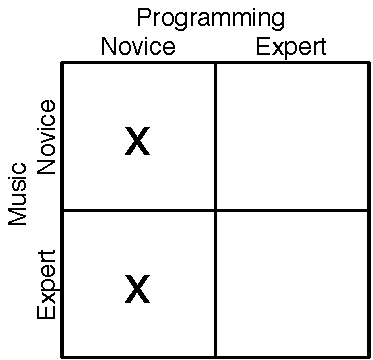
\includegraphics{2x2grid.pdf}
% \caption{Grid showing the targeted novice users}
% \label{fig:grid}
% \end{figure}

\section{Proposed solution}

\subsection{Slappability and Direct Combination}\label{slappability-and-direct-combination}

The development of software which is both usable to novice computer programmers and yet sufficiently expressive to allow for complex musical arrangements requires a suitable interaction framework. One interesting candidate is Direct Combination, a framework which derives from a user interface developed for a piece of music composition software.

Daniel Oppenheim initially developed \emph{Slappability} as an interaction framework for his DMIX music composition software (\citeyear{Oppenheim1994-zn}). The design allows for any object to act as the source; the user drags the source onto the target object. Once the mechanism is initiated any of the source object's characteristics can be applied to any of the target object's parameters. \emph{Direct Combination} (DC) is a development and generalisation of Slappability by Oppenheim and Simon Holland (\citeyear{Holland1999-zc}). DC allows users to select any number of interaction objects and uses this selection to constrain the search space of possible commands. In this way users can indicate which objects they wish to use without having to learn or remember the operations that the system allows. The selection of objects narrows options to those that are contextually relevant. DC is a suitable candidate for the proposed research activity due to its ability to accept input commands in many different orders \parencite{Holland2002-vc}, offering a good match for the spontaneous methodology often used in music composition \parencite{Collins2005-zk}. Users will not have to learn a potentially large number of operations in order to use the software; such operations can be abstract and therefore difficult to recall. The user will be able to select the objects they wish to manipulate and the system will constrain options to show only contextually relevant content.

The research also considers the concept of flow \parencite{Csikszentmihalyi2014-mh} as it considers the effect a carefully optimised experience can have on the user. It provides a useful framework in which to consider creativity, challenge and absorption. The tradeoff between expressivity and usability \parencite{Repenning1997-yv} will be an important aspect. 


\section{Methodology}
The chosen research method is a mixed methodology using an iterative research by design approach. This method requires the iterative creation and evaluation of algorithmic composition systems and their user interfaces to uncover issues, sharpen theory, and produce candidate solutions. An iterative series of interaction designs have been developed to implement this approach using expert inspection methods. A text-based DC implementation built in \emph{SuperCollider} has been taken through several iterations. The research will develop a range of prototypes which will be tested using a variety of software usability inspection methods. The results of the tests will provide hypotheses which will, in turn, inform subsequent iterations. This development cycle will repeat and lead to final stage prototypes which will be evaluated with end-users.



\section{Initial findings}
We began with an assumption, informed by an analytical review, that the software already in the space presents the inexperienced end user with a sub-optimal experience. To clarify this assumption a representative selection of algorithmic music software was analysed. The main findings were that existing software exhibited the following characteristics:

\begin{LaTeXdescription}
\item[Requires significant user knowledge] Much of the reviewed software requires the user to be competent in the design and implementation of algorithms within either text-oriented or graphical programming environments. A selection of software assumes musical knowledge, and some software requires the user to understand both areas.
\item[Use of metaphor] The use of metaphor is broadly applied in the area. Graphical programming languages make use of a patch-cable metaphor, while other software reference mixing desks, musical staff notation or sequencer-like piano rolls. Metaphor can be used to infer purpose and to leverage existing knowledge but it can also present a barrier to users with limited experience in the referenced fields.
\item[Imposes a defined working practice] Some reviewed software requires users to commit to a particular design which is subsequently difficult to change once the patch has become more complex.
\item[Lack of structural awareness] The user is not easily able to define, and subsequently change, the musical structure to be used in the composition. Users are able to create patches which express structure when using one of the reviewed programming languages but this requires significant programming knowledge.
\item[Complex visual design] The reviewed software exhibits a wide range of graphical design. Graphical programming languages, using a patching metaphor, allow complex operations but visibility is significantly reduced once the patch's size increases, leading to low juxtaposability. There are also issues with surfacing pertinent information and allowing the user to easily compare several elements.
\end{LaTeXdescription}


\section{Future work}

The goal of the project is to develop music composition software which is capable and engaging. The nature of music composition means that there are other constraints (such as the harmonic, melodic and rhythmic functionality). Given the problem under consideration a potentially useful match seems to be Direct Combination but, although this gives a principle, there are no guidelines for an application to music. Therefore, in order to find out the extent to which this makes algorithmic music composition engaging and to find out how DC should be applied it is necessary to carry out iterative design-based research.

\begin{LaTeXdescription}
\item[Pilot software testing] A review of candidate software platforms. Initial findings suggest that the software will be developed in \emph{SuperCollider} and will use Open Sound Control to connect the primitives, allowing for future expansion and interoperability.
\item[Research leading to personas] The intended user for the software is someone already familiar with music performance or software, and who is not skilled in programming. Matching users will be surveyed to create personas.
\item[Early development of alternative software prototypes] Software prototypes will be developed to test the findings from the paper prototyping stage. Initially, multiple potential designs will be developed in parallel and tested using a variety of software usability inspection methods in order to generate rich usability data in a short period of time. Each prototype will provide a hypothesis which will inform the next iteration. It is expected that some loose conclusions, assumptions and claims will be drawn from the variant tests.
\item[Development of the final stage prototype]
\emph{Software 1} will be the complete candidate software, including all DC functionality. \emph{Software 2} will be the control software with select DC functionality removed. This will allow for the effectiveness of the DC framework to be fully tested and considered.
\item[Empirical summative end-user studies] \label{end-user}
The final software design will be the source of two objective end-user tests. In the first test users will be observed using the software, with data collected on the number of musical constructs created in a given time, and on the complexity of models created. The second test will require a larger pool of users and will be used to validate findings from the first test and to facilitate the collection of an increased amount of objective data.
\end{LaTeXdescription}




% An example of a floating figure using the graphicx package.
% Note that \label must occur AFTER (or within) \caption.
% For figures, \caption should occur after the \includegraphics.
% Note that IEEEtran v1.7 and later has special internal code that
% is designed to preserve the operation of \label within \caption
% even when the captionsoff option is in effect. However, because
% of issues like this, it may be the safest practice to put all your
% \label just after \caption rather than within \caption{}.
%
% Reminder: the "draftcls" or "draftclsnofoot", not "draft", class
% option should be used if it is desired that the figures are to be
% displayed while in draft mode.
%
%\begin{figure}[!t]
%\centering
%\includegraphics[width=2.5in]{myfigure}
% where an .eps filename suffix will be assumed under latex, 
% and a .pdf suffix will be assumed for pdflatex; or what has been declared
% via \DeclareGraphicsExtensions.
%\caption{Simulation Results}
%\label{fig_sim}
%\end{figure}

% Note that IEEE typically puts floats only at the top, even when this
% results in a large percentage of a column being occupied by floats.


% An example of a double column floating figure using two subfigures.
% (The subfig.sty package must be loaded for this to work.)
% The subfigure \label commands are set within each subfloat command, the
% \label for the overall figure must come after \caption.
% \hfil must be used as a separator to get equal spacing.
% The subfigure.sty package works much the same way, except \subfigure is
% used instead of \subfloat.
%
%\begin{figure*}[!t]
%\centerline{\subfloat[Case I]\includegraphics[width=2.5in]{subfigcase1}%
%\label{fig_first_case}}
%\hfil
%\subfloat[Case II]{\includegraphics[width=2.5in]{subfigcase2}%
%\label{fig_second_case}}}
%\caption{Simulation results}
%\label{fig_sim}
%\end{figure*}
%
% Note that often IEEE papers with subfigures do not employ subfigure
% captions (using the optional argument to \subfloat), but instead will
% reference/describe all of them (a), (b), etc., within the main caption.


% An example of a floating table. Note that, for IEEE style tables, the 
% \caption command should come BEFORE the table. Table text will default to
% \footnotesize as IEEE normally uses this smaller font for tables.
% The \label must come after \caption as always.
%
%\begin{table}[!t]
%% increase table row spacing, adjust to taste
%\renewcommand{\arraystretch}{1.3}
% if using array.sty, it might be a good idea to tweak the value of
% \extrarowheight as needed to properly center the text within the cells
%\caption{An Example of a Table}
%\label{table_example}
%\centering
%% Some packages, such as MDW tools, offer better commands for making tables
%% than the plain LaTeX2e tabular which is used here.
%\begin{tabular}{|c||c|}
%\hline
%One & Two\\
%\hline
%Three & Four\\
%\hline
%\end{tabular}
%\end{table}


% Note that IEEE does not put floats in the very first column - or typically
% anywhere on the first page for that matter. Also, in-text middle ("here")
% positioning is not used. Most IEEE journals/conferences use top floats
% exclusively. Note that, LaTeX2e, unlike IEEE journals/conferences, places
% footnotes above bottom floats. This can be corrected via the \fnbelowfloat
% command of the stfloats package.



% conference papers do not normally have an appendix


% use section* for acknowledgement
% \section*{Acknowledgment}
% 
% The authors would like to thank...





% trigger a \newpage just before the given reference
% number - used to balance the columns on the last page
% adjust value as needed - may need to be readjusted if
% the document is modified later
%\IEEEtriggeratref{8}
% The "triggered" command can be changed if desired:
%\IEEEtriggercmd{\enlargethispage{-5in}}

% references section

\printbibliography[title=References]

% can use a bibliography generated by BibTeX as a .bbl file
% BibTeX documentation can be easily obtained at:
% http://www.ctan.org/tex-archive/biblio/bibtex/contrib/doc/
% The IEEEtran BibTeX style support page is at:
% http://www.michaelshell.org/tex/ieeetran/bibtex/
%\bibliographystyle{IEEEtran}
% argument is your BibTeX string definitions and bibliography database(s)
%\bibliography{IEEEabrv,../bib/paper}
%
% <OR> manually copy in the resultant .bbl file
% set second argument of \begin to the number of references
% (used to reserve space for the reference number labels box)
% \begin{thebibliography}{1}
% 
% \bibitem{IEEEhowto:kopka}
% H.~Kopka and P.~W. Daly, \emph{A Guide to \LaTeX}, 3rd~ed.\hskip 1em plus
%   0.5em minus 0.4em\relax Harlow, England: Addison-Wesley, 1999.
% 
% \end{thebibliography}




% that's all folks
\end{document}


